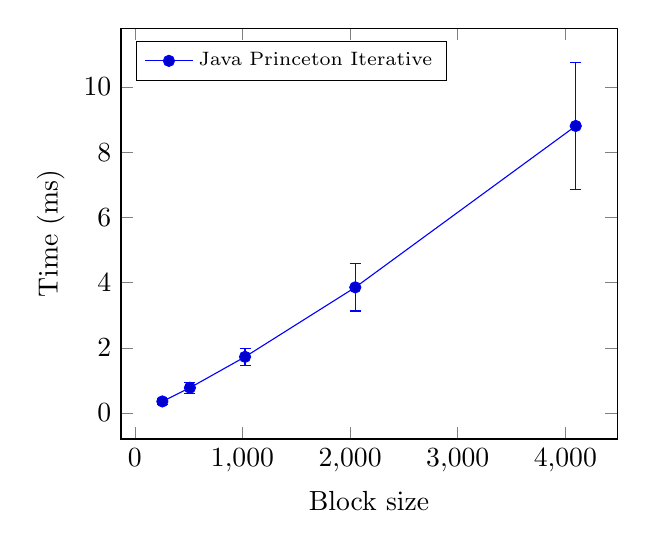
\begin{tikzpicture}
\begin{axis}[xlabel={Block size},ylabel={Time (ms)},width=0.65\linewidth,legend pos=north west,scaled y ticks = false,legend cell align=left,legend style={font=\scriptsize}]
\addplot+[error bars/.cd, y dir=both,y explicit] coordinates {
(256, 0.3547) +- (0.1008, 0.1008)
(512, 0.7740) +- (0.1657, 0.1657)
(1024, 1.7228) +- (0.2675, 0.2675)
(2048, 3.8546) +- (0.7268, 0.7268)
(4096, 8.8053) +- (1.9485, 1.9485)
};
\legend{Java Princeton Iterative}
\end{axis}
\end{tikzpicture}
